%%%%%%%%%%%%%%%%%%%%%%%%%%%%%%%%%%%%%%%%%
% Jacobs Landscape Poster
% LaTeX Template
% Version 1.0 (29/03/13)
%
% Created by:
% Computational Physics and Biophysics Group, Jacobs University
% https://teamwork.jacobs-university.de:8443/confluence/display/CoPandBiG/LaTeX+Poster
% 
% Further modified by:
% Nathaniel Johnston (nathaniel@njohnston.ca)
%
% This template has been downloaded from:
% http://www.LaTeXTemplates.com
%
% License:
% CC BY-NC-SA 3.0 (http://creativecommons.org/licenses/by-nc-sa/3.0/)
%
%%%%%%%%%%%%%%%%%%%%%%%%%%%%%%%%%%%%%%%%%

%----------------------------------------------------------------------------------------
%	PACKAGES AND OTHER DOCUMENT CONFIGURATIONS
%----------------------------------------------------------------------------------------

\documentclass[final]{beamer}

\usepackage[scale=1.15]{beamerposter} % Use the beamerposter package for laying out the poster

\usetheme{confposter} % Use the confposter theme supplied with this template

\setbeamercolor{block title}{fg=ngreen,bg=white} % Colors of the block titles
\setbeamercolor{block body}{fg=black,bg=white} % Colors of the body of blocks
\setbeamercolor{block alerted title}{fg=white,bg=dblue!70} % Colors of the highlighted block titles
\setbeamercolor{block alerted body}{fg=black,bg=dblue!10} % Colors of the body of highlighted blocks
% Many more colors are available for use in beamerthemeconfposter.sty

%-----------------------------------------------------------
% Define the column widths and overall poster size
% To set effective sepwid, onecolwid and twocolwid values, first choose how many columns you want and how much separation you want between columns
% In this template, the separation width chosen is 0.024 of the paper width and a 4-column layout
% onecolwid should therefore be (1-(# of columns+1)*sepwid)/# of columns e.g. (1-(4+1)*0.024)/4 = 0.22
% Set twocolwid to be (2*onecolwid)+sepwid = 0.464
% Set threecolwid to be (3*onecolwid)+2*sepwid = 0.708

\newlength{\sepwid}
\newlength{\onecolwid}
\newlength{\twocolwid}
\newlength{\threecolwid}
\setlength{\paperwidth}{48in} % A0 width: 46.8in
\setlength{\paperheight}{36in} % A0 height: 33.1in
\setlength{\sepwid}{0.024\paperwidth} % Separation width (white space) between columns
\setlength{\onecolwid}{0.22\paperwidth} % Width of one column
\setlength{\twocolwid}{0.464\paperwidth} % Width of two columns
\setlength{\threecolwid}{0.708\paperwidth} % Width of three columns
\setlength{\topmargin}{-0.5in} % Reduce the top margin size
%-----------------------------------------------------------

\usepackage{graphicx}  % Required for including images

\usepackage{booktabs} % Top and bottom rules for tables

%----------------------------------------------------------------------------------------
%	TITLE SECTION 
%----------------------------------------------------------------------------------------

\title{Towards Hierarchical Importance Attribution: Explaining Compositional Semantics for Neural Sequence Models \texorpdfstring{\cite{jin2020towards}}} % Poster title

\author{Reviewed by Sara Amrouche, Roger Lucena and Alexandre Macedo} % Author(s)

\institute{Sorbonne University, Paris VI} % Institution(s)

%----------------------------------------------------------------------------------------

\begin{document}

\addtobeamertemplate{block end}{}{\vspace*{2ex}} % White space under blocks
\addtobeamertemplate{block alerted end}{}{\vspace*{2ex}} % White space under highlighted (alert) blocks

\setlength{\belowcaptionskip}{2ex} % White space under figures
\setlength\belowdisplayshortskip{2ex} % White space under equations

\begin{frame}[t] % The whole poster is enclosed in one beamer frame
\begin{columns}[t] % The whole poster consists of three major columns, the second of which is split into two columns twice - the [t] option aligns each column's content to the top

\begin{column}{\sepwid}\end{column} % Empty spacer column

\begin{column}{\onecolwid} % The first column

%----------------------------------------------------------------------------------------
%	OBJECTIVES
%----------------------------------------------------------------------------------------
\begin{alertblock}{Objectives}

\begin{itemize}
\item Tackle the problem of \textbf{post-hoc hierarchical explanations} to understand how models, even black-box ones, handle compositional semantics (such as negation or stress);

\item Highlight, in this context, \textbf{key properties} for measuring importance of words and phrases, in special \textbf{non-additivity} and \textbf{context-independence}, and propose a mathematically sound way to quantify them;

\item Introduce, from this proposed formulation, \textbf{two explanation algorithms};

\item \textbf{Test and compare} those algorithms with the state-of-the-art in the field, both quantitatively and qualitatively, keeping track of how they improve \textbf{human trust} of model as well. 
\end{itemize}

\end{alertblock}

%----------------------------------------------------------------------------------------
%	INTRODUCTION
%----------------------------------------------------------------------------------------
\begin{block}{Introduction and Outline}

% Following the formulation, we propose Sampling and Contextual Decomposition (SCD) algorithm and Sampling and Occlusion (SOC) algorithm

%(1) we identify the key challenges in generating post-hoc hierarchical explanations and propose a mathematically sound way to quantify context independent importance of words and phrases for generating hierarchical explanations; (2) we extend previous post-hoc explanation algorithm based on the new formulation of N-context independent importance and develop two effective hierarchical explanation algorithms; and (3) both experiments using automatic evaluation metrics and human evaluation demonstrate that the proposed explanation algorithms consistently outperform the compared methods (with both LSTM and Transformer as base models) over several datasets.

%non-additive and context-independent importance for individual words and phrases

%by identifying desired properties of phrase-level importance score attribution for hierarchical explanations. We propose a measure of context-independent importance of a phrase and introduce two explanation algorithms instantiated from the proposed formulation.

Deep neural networks have proved themselves extremely good for handling complicated semantics in natural language. Nevertheless, they are mostly seen as black box solutions. To understand how models handle compositional semantics the authors decided to tackle the problem of hierarchical explanations. 

They start by identifying that the key challenge is to compute non-additive and context-independent importance for individual words and phrases. They show, along the paper, that prior efforts on the domain, such as Contextual Decomposition (CD), do not satisfy these properties mathematically - which leads to inconsistent explanation quality in different models.   

Then, they propose two algorithms for quantifying the importance of words and phrases to generate hierarchical explanations. The first one, \textbf{Sampling and Contextual Decomposition (SCD)}, is obtained after modifications over CD, following their formulation. The second one is a simpler and model-agnostic algorithm called \textbf{Sampling and OCclusion (SOC)}, with competitive performance. Comparable to the state-of-the-art on multiple datasets, they are also shown to help extract classification rules and improve human trust of models.

%Comparable to the state-of-the-art on multiple datasets, they show their methods help not only explain compositionality of semantics, but also 

%----------------------------------------------------------------------------------------
%	LOGO
%----------------------------------------------------------------------------------------
\vspace{17pt}
\begin{center}
        
\includegraphics[width=0.26\linewidth]{images/logo-sciences-sorbonne-universit.png}
\end{center}

\end{block}

\end{column} % End of the first column

\begin{column}{\sepwid}\end{column} % Empty spacer column

\begin{column}{\twocolwid} % Begin a column which is two columns wide (column 2)
\begin{columns}[t,totalwidth=\twocolwid] % Split up the two columns wide column
\begin{column}{\onecolwid}\vspace{-.6in} % The first column within column 2 (column 2.1)
% XXXXXXXXXXXX|
% XXXXXXXXXXXX|_____________
%             |
%             |
%----------------------------------------------------------------------------------------
%	PRINCIPLES


%----------------------------------------------------------------------------------------
\begin{block}{Principles}

Being $x_{i:T}$ a sequence of low-dimensional word embeddings (the input), represented as $x$ for brevity, and $p$ a phrase (or word), we have that the two key properties can be expressed as follows:

\begin{itemize}
    \item \textbf{Non-additivity:}
    
    The importance of a phrase, given by $\phi(p, x)$, should be quantified by a non-linear function over the importance scores of all the component words $x_i \in p$, i.e.:
    
    \begin{equation}
        \phi(p, x) \neq \sum _{x_i \in p} \phi(x_i, x) 
    \end{equation}
    
    \item \textbf{Context-independence:}
    
    % Considering how combining two phrases $p_1$ and $p_2$ contribute to a specific prediction for an input $x$, we expect that for input sentences $\hat{x}$, where only $p_2$ is replaced to another phrase, the importance attribution for $p_1$ remains the same, i.e.: 
    
    % \begin{equation}
    %     \phi(p_1, x) = \phi(p_1, \hat{x}) 
    % \end{equation}
    
    If we consider a phrase $p$ in $x$ and change some contextual words or phrases around it in the input $x$, obtaining $\hat{x}$, we expect that the importance attribution for $p$ remains the same, i.e.:
    
    \begin{equation}
        \phi(p, x) = \phi(p, \hat{x}) 
    \end{equation}
    
    From this property is born the idea of sampling the context, at the core of SCD and SOC.
\end{itemize}

Some prior methods, such as Contextual Decomposition and Agglomerative Contextual Decomposition (ACD), fail to attend these desired properties.

% TODO: Explain the idea of CD and why it is not good, using beta and gamma and so on.


\end{block}

\end{column} % End of column 2.1
\begin{column}{\onecolwid}\vspace{-.6in} % The second column within column 2 (column 2.2)
%             |XXXXXXXXXXXXX
% ____________|XXXXXXXXXXXXX
%             |
%             |
%----------------------------------------------------------------------------------------
%	METHODS
%----------------------------------------------------------------------------------------
\begin{block}{Methods}

\begin{itemize}
    \item \textbf{Sampling and Contextual Decomposition algorithm:}
    SCD modifies the way to decompose activation functions in CD.
    \begin{equation}
     \beta^{\prime} = \mathbb{E}_{\gamma}[\sigma ( \beta + \gamma )- \sigma(\gamma)] = \mathbb{E}_{h}[\sigma(\textbf{h}) -\sigma(\textbf{h} - \beta)]
    \end{equation}
     \begin{figure}
        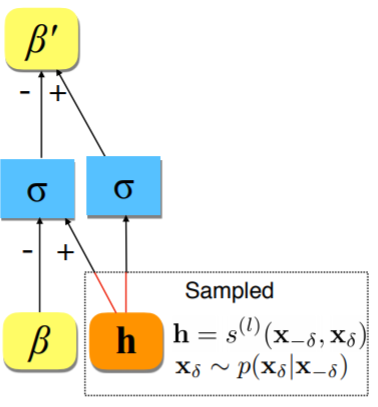
\includegraphics[width=0.35\linewidth]{images/SCD.png}
        \caption{Visualization of decomposition using SCD}
    \end{figure}
    They first pretrain an \textit{LSTM} from two directions on the training data. For sampling they mask the words that are not conditioned in \textit{p}$(x_\delta\|x_{-\delta})$ or perform Gibbs sampling.
    
    
    \item \textbf{Sampling and OCclusion algorithm:}
    Similarly to SCD, SOC samples neighboring words $x_\gamma$ from a trained language and obtain a set of neighboring word replacements $S$. For each replacement, it computes the model prediction differences after replacing a phrase $p$ with padding tokens. Formally we have the equation: \newline
     \begin{equation}
     \phi(p, x) = \frac{1}{S} \sum_{x_\delta \in S} [ s(x_{-\delta};x_\delta)
    - s(x_{-\{\delta,p\}}; x_\delta; \textbf{0}_p)]
     \end{equation}
\end{itemize}
\end{block}

\end{column} % End of column 2.2
\end{columns} % End of the split of column 2 - any content after this will now take up 2 columns width

%----------------------------------------------------------------------------------------
%	Middle banner
%----------------------------------------------------------------------------------------
\begin{alertblock}{Main Result}
    \begin{figure}
        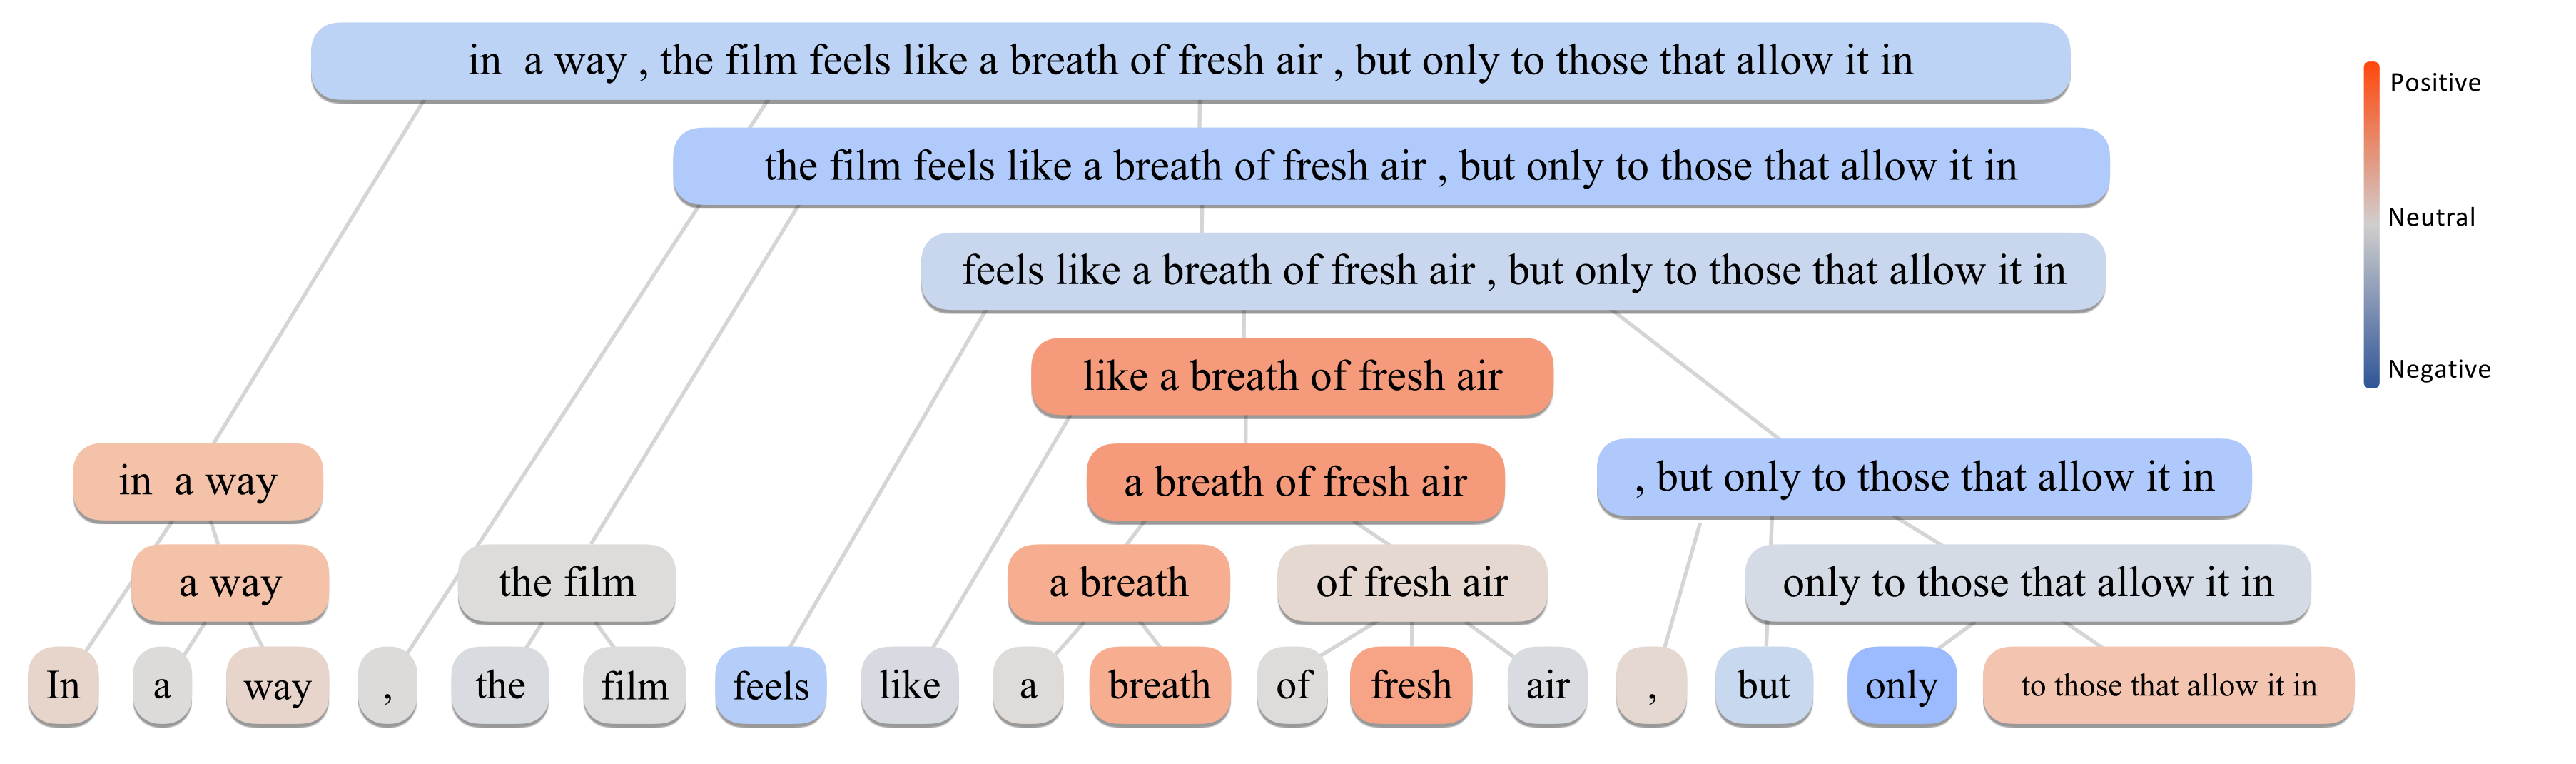
\includegraphics[width=0.95\linewidth]{images/result.png}
        \caption{Hierarchical Explanation of a prediction made by the BERT Transformer model on SST-2. Taken from \cite{jin2020towards}}
    \end{figure}
\end{alertblock} 

\begin{columns}[t,totalwidth=\twocolwid] % Split up the two columns wide column again
\begin{column}{\onecolwid} % The first column within column 2 (column 2.1)
%             |
% ____________|_____________
% XXXXXXXXXXXX|
% XXXXXXXXXXXX|



\end{column} % End of column 2.1

\begin{column}{\onecolwid} % The second column within column 2 (column 2.2)
%             |
% ____________|_____________
%             |XXXXXXXXXXXXX
%             |XXXXXXXXXXXXX

\end{column} % End of column 2.2
\end{columns} % End of the split of column 2
\end{column} % End of the second column

\begin{column}{\sepwid}\end{column} % Empty spacer column

\begin{column}{\onecolwid} % The third column
%----------------------------------------------------------------------------------------
%	RESULTS
%----------------------------------------------------------------------------------------
\begin{block}{Results}

% After a contact with the authors, we decided to focus on the SOC algorithm.

As proposed in \cite{jin2020towards}, we adapted the work of \cite{wang2019bert} to use BERT for sampling. To illustrate, given the input "countryside around her" the sampled context would be: 

\begin{quote}
    "only a handful of beasts neared her . with the \textbf{countryside around her} she couldn't see where she might find them .". 
\end{quote}


% \begin{figure}
%     
\includegraphics[width=0.8\linewidth]{images/placeholder.jpg}
%     \caption{Figure caption}
% \end{figure}

Also, we adapted the work of \cite{clairett2018} for implementing the Occlusion algorithm in the context of Importance Attribution. To illustrate again, take the input below:

\begin{quote}
    \textbf{"The film is faithful to what one presumes are the book's twin premises: that we become who we are on the backs of our parents,} but we have no idea who they were at our age and that time is a fleeting and precious commodity no matter how old you are."
\end{quote}

It is classified with the label "positive" by the LSTM. Considering the highlighted phrase, the model prediction score (in the space of log probabilities) is $-0.59$ before occlusion, and $-0.84$ after. This shows how this phrase has a relevant positive contribution (+0.25) into the model prediction, as expected.

% If we compute the model prediction score differences between the original and the highlighted phrase above replaced by padding tokens, we verify a positive difference of $0.24$ in the space of log probabilities, with the initial scores being on the order of $0.6$ and $0.8$. This indicates that, as expected, the highlighted phrase has a relevant contribution to the final model prediction.  

\end{block}

%----------------------------------------------------------------------------------------
%	CONCLUSION
%----------------------------------------------------------------------------------------
\begin{block}{Conclusion}
It was interesting to see how important the sampling step was for achieving the desired properties highlighted before and for expanding the state-of-the-art. Also, the attention given to the human trust on the paper was appreciable. 


\end{block}

%----------------------------------------------------------------------------------------
%	ADDITIONAL INFORMATION
%----------------------------------------------------------------------------------------

% \begin{block}{Additional Information}

% Maecenas ultricies feugiat velit non mattis. Fusce tempus arcu id ligula varius dictum. 
% \begin{itemize}
% \item Curabitur pellentesque dignissim
% \item Eu facilisis est tempus quis
% \item Duis porta consequat lorem
% \end{itemize}

% \end{block}
%----------------------------------------------------------------------------------------
%	REFERENCES
%----------------------------------------------------------------------------------------
\begin{block}{References}

% \nocite{*} % Insert publications even if they are not cited in the poster
\small{\bibliographystyle{abbrv}
\bibliography{sample}\vspace{0.75in}}

\end{block}

%----------------------------------------------------------------------------------------
%	ACKNOWLEDGEMENTS
%----------------------------------------------------------------------------------------

% \setbeamercolor{block title}{fg=red,bg=white} % Change the block title color

% \begin{block}{Acknowledgements}

% \small{\rmfamily{Nam mollis tristique neque eu luctus. Suspendisse rutrum congue nisi sed convallis. Aenean id neque dolor. Pellentesque habitant morbi tristique senectus et netus et malesuada fames ac turpis egestas.}} \\

% \end{block}

%----------------------------------------------------------------------------------------
%	CONTACT INFORMATION
%----------------------------------------------------------------------------------------

% \setbeamercolor{block alerted title}{fg=black,bg=norange} % Change the alert block title colors
% \setbeamercolor{block alerted body}{fg=black,bg=white} % Change the alert block body colors

% \begin{alertblock}{Contact Information}

% \begin{itemize}
% \item Web: \href{http://www.university.edu/smithlab}{http://www.university.edu/smithlab}
% \item Email: \href{mailto:john@smith.com}{john@smith.com}
% \item Phone: +1 (000) 111 1111
% \end{itemize}

% \end{alertblock}


\end{column} % End of the third column
\end{columns} % End of all the columns in the poster
\end{frame} % End of the enclosing frame

\end{document}
